%%% BEN 5' %%%

\section{Allgemeine Grundlagen}

\subsection{Die Hyperfeinstruktur}

\begin{frame}
\frametitle{Hyperfeinstruktur-Aufspaltung}
\begin{itemize}
    \item<1-> Kopplung von Kernspin $\vec{I}$ und elektronischem Gesamtdrehimpuls $\vec{J}$
    \begin{equation*}
        \vec{F} = \vec{I} + \vec{J} \qquad \qquad \abs{I - J} \leq F \leq \abs{I + J}
    \end{equation*}
    \item<2-> Energieaufspaltung
    \begin{equation*}
        \Delta E_\text{HFS} = - \vec{\mu}_I \cdot \vec{B}_J
    \end{equation*}
    \item<3-> Für benachbarte Energieniveaus
    \begin{equation*}
        \Delta E_{\Delta F = 1} (F) = A(F+1)
    \end{equation*}
    Intervallkonstante $A$
\end{itemize}
\end{frame}


\begin{frame}
\frametitle{Hyperfeinstruktur-Aufspaltung}
%TODO Termschema ohne Zeeman?
\setbeamerfont{myfont}{size*=45}
\usebeamerfont{myfont}

\begin{figure}
    \centering
    \def\svgwidth{0.45\textwidth}
    \input{../img/termschema.pdf_tex}
    %\caption{Termschemata der beiden Rubidiumisotope:
    %Feinstruktur, Hyperfeinstruktur und Zeeman-Aufspaltung der D$_1$-Linie im äußeren Magnetfeld.}
    \label{img:termschema}
\end{figure}
\end{frame}

\begin{frame}
\frametitle{Spektrallinien}
\begin{figure}
    \centering
    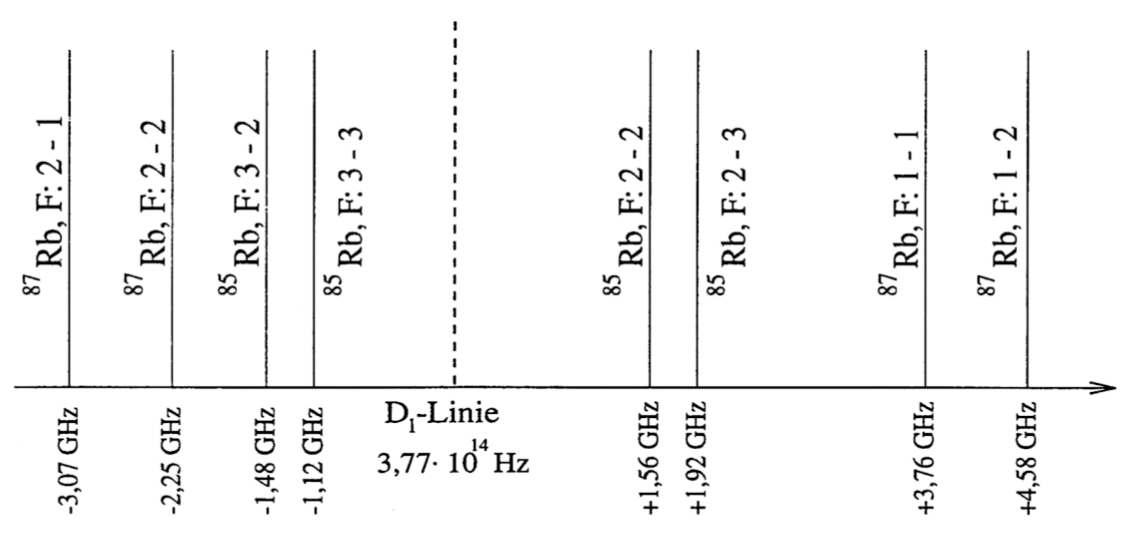
\includegraphics[width=\textwidth]{../img/HFSspect_theo.png}
    \caption{Spektrallinien der Hyperfeinstruktur des ${}^2\text{S}_{1/2}$\,-\,${}^2\text{P}_{1/2}$\,-\,Übergangs
    von \rb{85} und \rb{87}.}  % TODO Inkscape oder ref
\end{figure}
\end{frame}

\begin{frame}
\frametitle{Zeeman-Aufspaltung der Hyperfeinstruktur}
\begin{itemize}
    \item<1-> ohne Magnetfeld: Niveau ist $(2F+1)$-fach entartet
    \begin{equation*}
        F_z = m_F \hbar \qquad \qquad -F \leq m_F \leq F
    \end{equation*}
    \item<2-> mit äußerem Magnetfeld $\vec{B}_0$: Zeeman-Aufspaltung
    \item<3-> Für benachbarte Energieniveaus
    \begin{equation*}
        \Delta E_\text{HFS}^\text{Zeeman}(\Delta m_F = 1) = \frac{g_J}{2 \left( I + \frac{1}{2} \right) } \mu_B B_0
    \end{equation*}
    Bohrsches Magneton $\mu_B$, Landé-Faktor $g_J$
\end{itemize}
\end{frame}

\begin{frame}
\frametitle{Zeeman-Aufspaltung der Hyperfeinstruktur}
\setbeamerfont{myfont}{size*=45}
\usebeamerfont{myfont}

\begin{figure}
    \centering
    \def\svgwidth{0.45\textwidth}
    \input{../img/termschema.pdf_tex}
    \caption{Termschema.}
\end{figure}
\end{frame}




%%% MORITZ 2.5' %%%

\subsection{Laser}



\begin{frame}
\frametitle{Laser - Aufbau}

\setbeamerfont{myfont}{size*=80}
\usebeamerfont{myfont}
\begin{figure}
    \centering
    \def\svgwidth{\textwidth}
    \input{../img/aufbauLaser.pdf_tex}
    \caption{Aufbau zur Messung der $P$-$I$-Kennlinie der Laserdiode.}
\end{figure}

\end{frame}






\begin{frame}
\frametitle{$P$-$I$-Kennlinie}

\begin{figure}[H]
    \begin{center}
        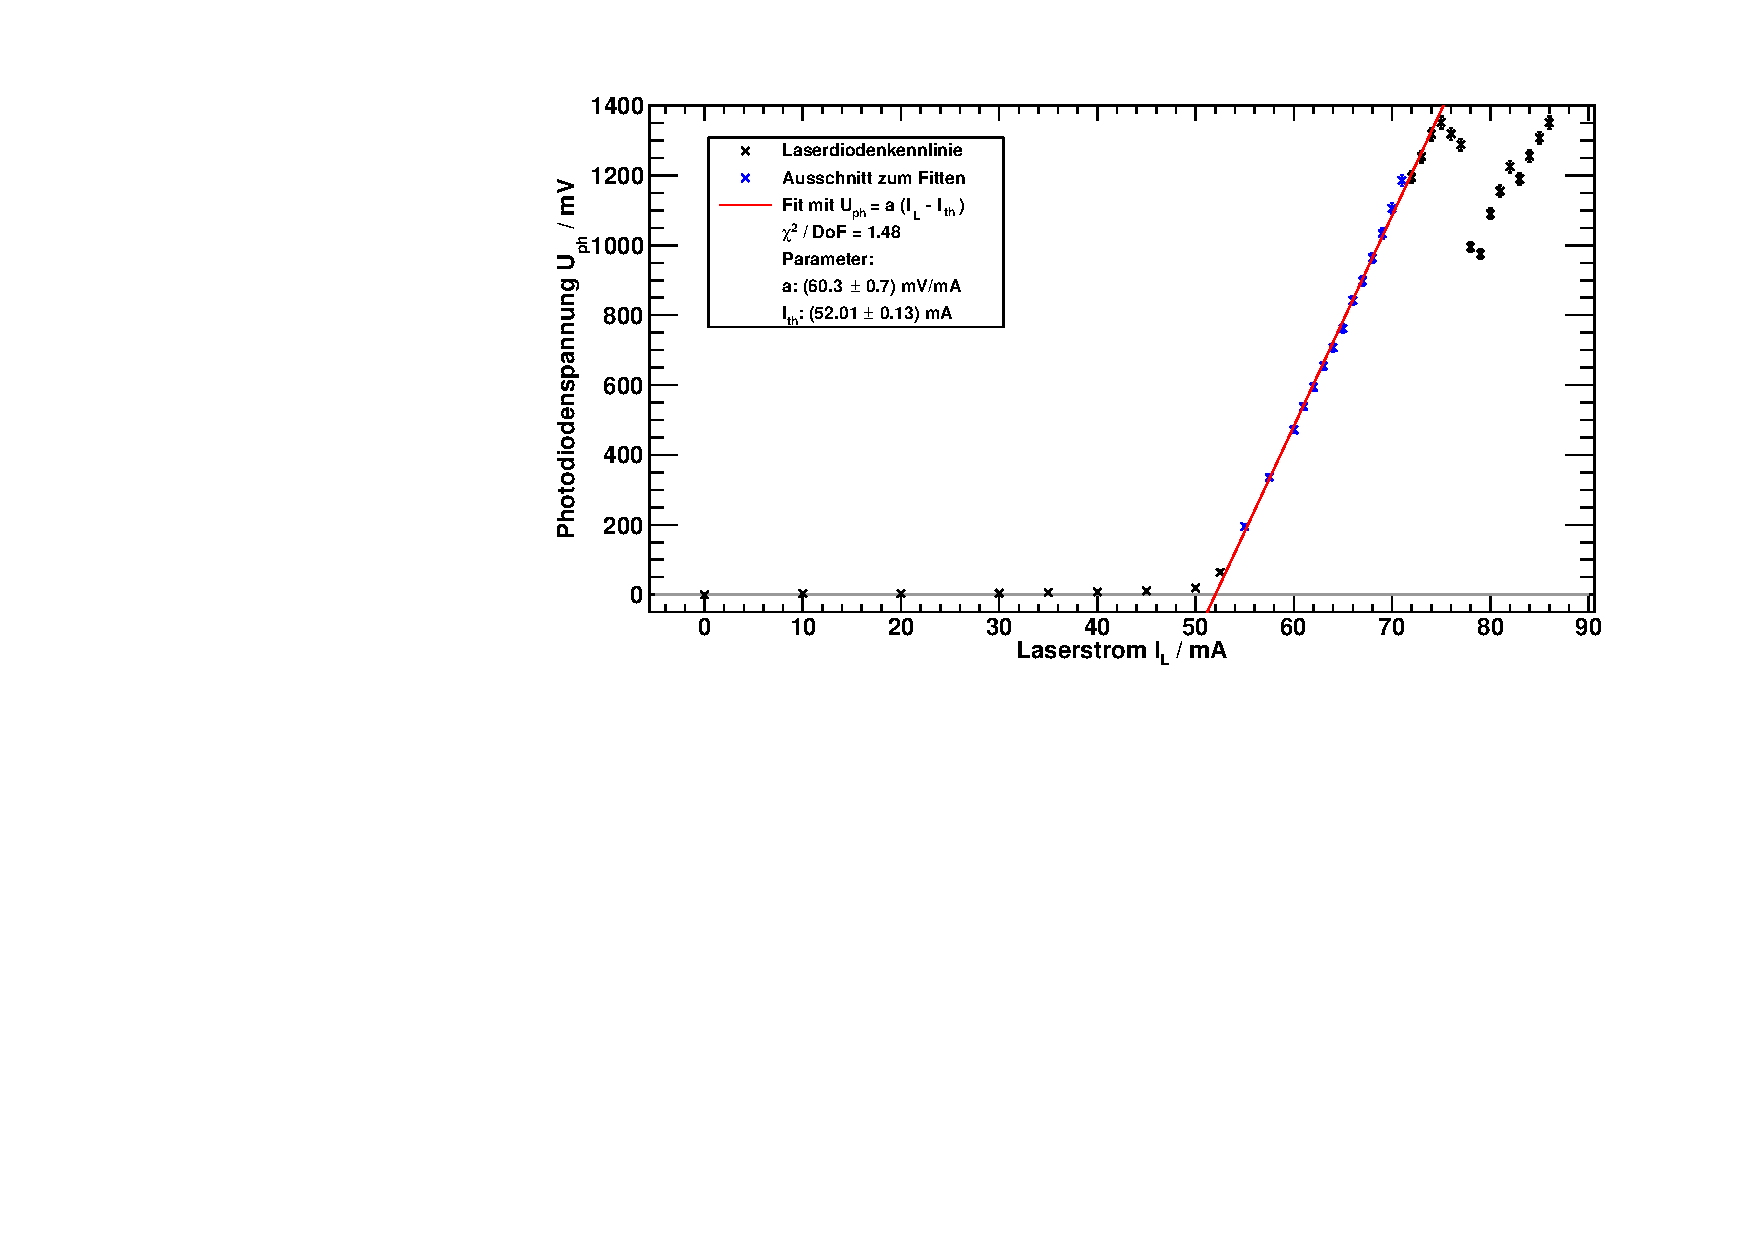
\includegraphics[width=\textwidth]{../img/diodenkennlinie.pdf}
        \caption{$P$-$I$-Kennlinie der im Versuch verwendeten Laserdiode.}
    \end{center}
\end{figure}



\end{frame}


\begin{frame}
\frametitle{Laser - Aufbau}

\setbeamerfont{myfont}{size*=80}
\usebeamerfont{myfont}
\begin{figure}
    \centering
    \def\svgwidth{\textwidth}
    \input{../img/aufbauEtalon.pdf_tex}
    \caption{Aufbau zur Identifikation von Modensprüngen der Laserdiode.}
\end{figure}
\usebeamerfont{standard}

\begin{itemize}
  \item \textbf{Etalon:} Transmissionsmaxima mit bekanntem Abstand
\end{itemize}

\end{frame}


\begin{frame}
\frametitle{Etalon - Modensprung}

\begin{figure}[H]
    \begin{center}
        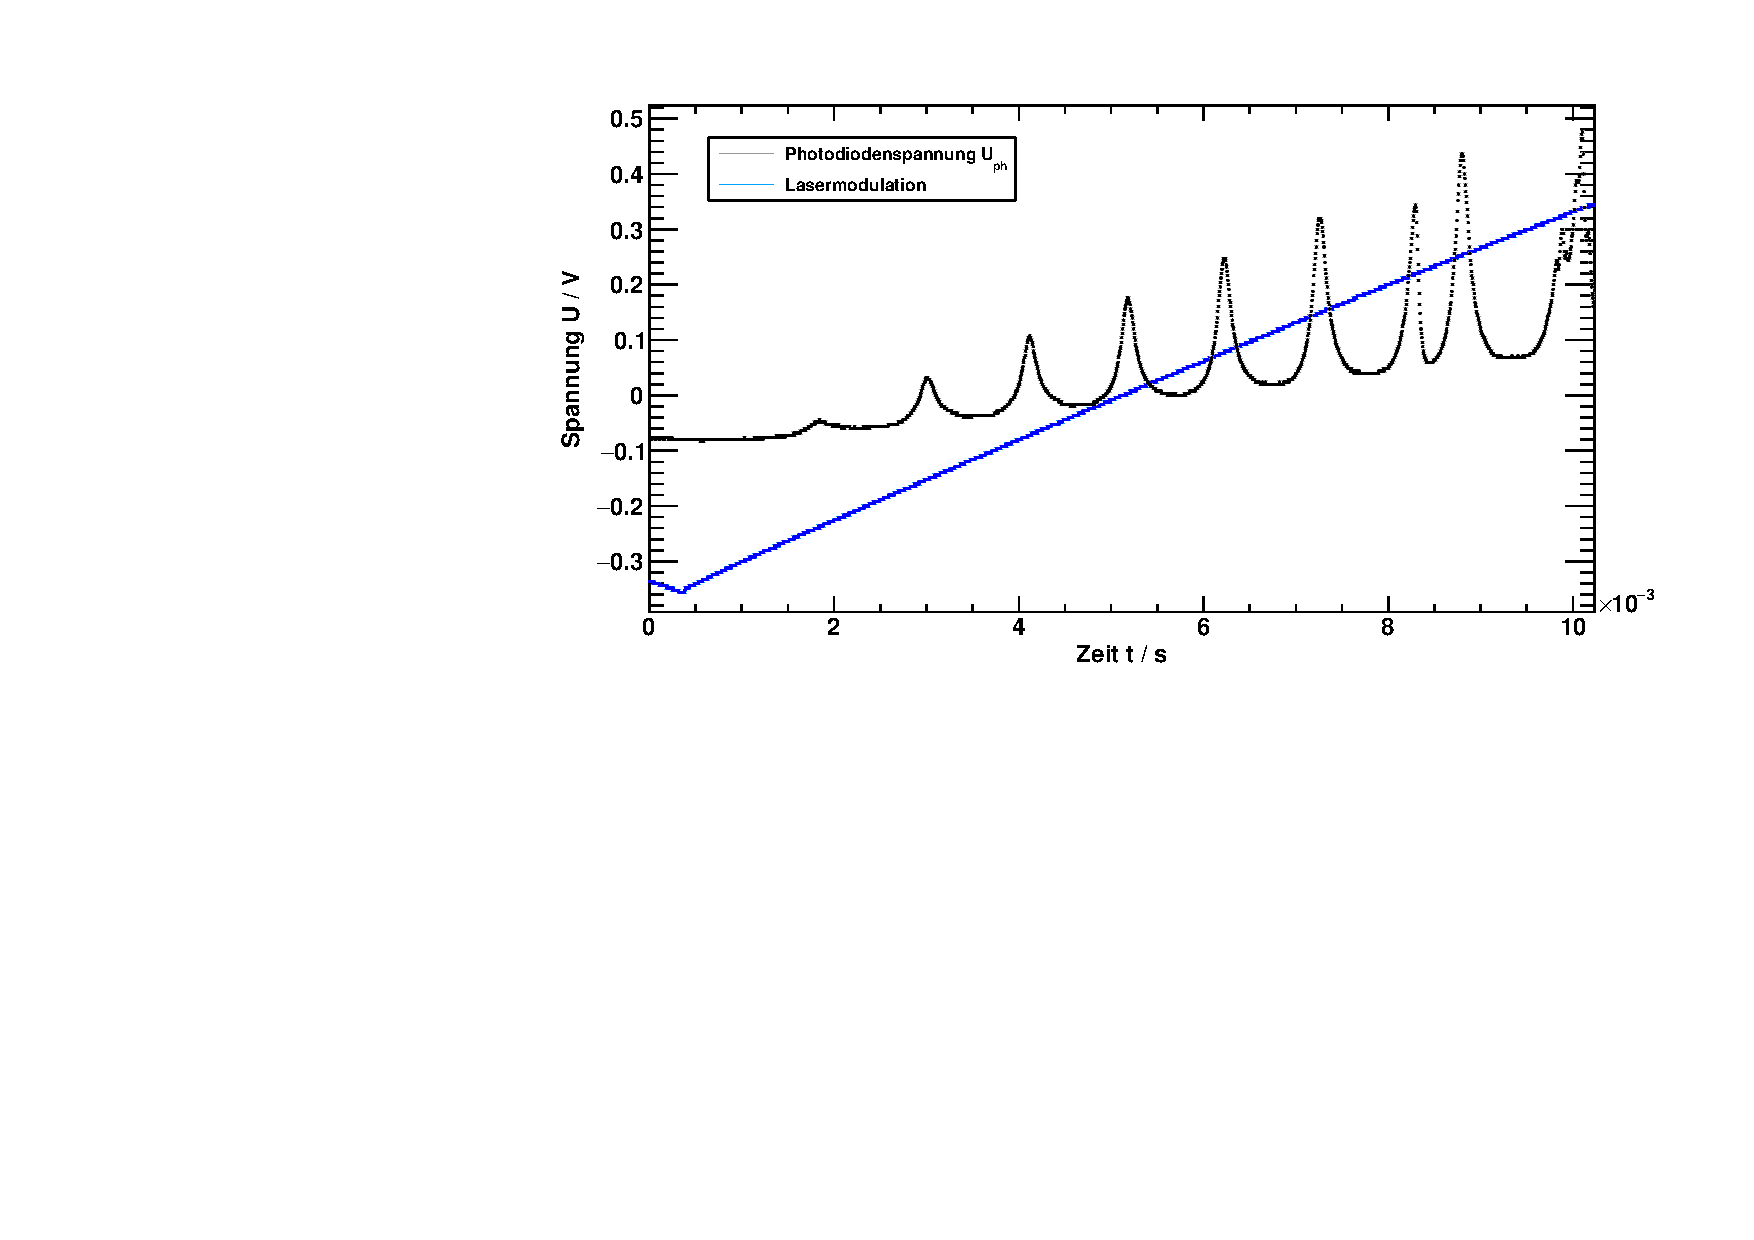
\includegraphics[width=\textwidth]{../img/up-etalon_zoom.pdf}
        \caption{caption.}
    \end{center}
\end{figure}


\end{frame}
